\documentclass[14pt]{extbook}
\usepackage{multicol, enumerate, enumitem, hyperref, color, soul, setspace, parskip, fancyhdr} %General Packages
\usepackage{amssymb, amsthm, amsmath, latexsym, units, mathtools} %Math Packages
\everymath{\displaystyle} %All math in Display Style
% Packages with additional options
\usepackage[headsep=0.5cm,headheight=12pt, left=1 in,right= 1 in,top= 1 in,bottom= 1 in]{geometry}
\usepackage[usenames,dvipsnames]{xcolor}
\usepackage{dashrule}  % Package to use the command below to create lines between items
\newcommand{\litem}[1]{\item#1\hspace*{-1cm}\rule{\textwidth}{0.4pt}}
\pagestyle{fancy}
\lhead{Progress Quiz 7}
\chead{}
\rhead{Version C}
\lfoot{3510-5252}
\cfoot{}
\rfoot{Summer C 2021}
\begin{document}

\begin{enumerate}
\litem{
Construct the lowest-degree polynomial given the zeros below. Then, choose the intervals that contain the coefficients of the polynomial in the form $ax^3+bx^2+cx+d$.\[ \frac{7}{4}, \frac{-7}{5}, \text{ and } \frac{5}{2} \]\begin{enumerate}[label=\Alph*.]
\item \( a \in [39, 49], b \in [114, 119], c \in [-65, -62], \text{ and } d \in [-247, -238] \)
\item \( a \in [39, 49], b \in [-87, -83], c \in [-137, -129], \text{ and } d \in [241, 248] \)
\item \( a \in [39, 49], b \in [-115, -112], c \in [-65, -62], \text{ and } d \in [241, 248] \)
\item \( a \in [39, 49], b \in [-115, -112], c \in [-65, -62], \text{ and } d \in [-247, -238] \)
\item \( a \in [39, 49], b \in [25, 29], c \in [-220, -214], \text{ and } d \in [-247, -238] \)

\end{enumerate} }
\litem{
Describe the zero behavior of the zero $x = -8$ of the polynomial below.\[ f(x) = 3(x + 7)^{11}(x - 7)^{9}(x - 8)^{8}(x + 8)^{5} \]\begin{enumerate}[label=\Alph*.]
\begin{multicols}{2}\item 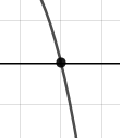
\includegraphics[width = 0.3\textwidth]{../Figures/polyZeroBehaviorCopyAC.png}\item 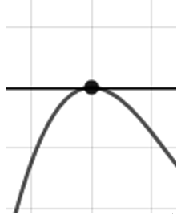
\includegraphics[width = 0.3\textwidth]{../Figures/polyZeroBehaviorCopyBC.png}\item 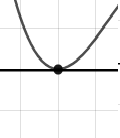
\includegraphics[width = 0.3\textwidth]{../Figures/polyZeroBehaviorCopyCC.png}\item 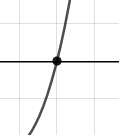
\includegraphics[width = 0.3\textwidth]{../Figures/polyZeroBehaviorCopyDC.png}\end{multicols}\item None of the above.
\end{enumerate} }
\litem{
Which of the following equations \textit{could} be of the graph presented below?
\begin{center}
    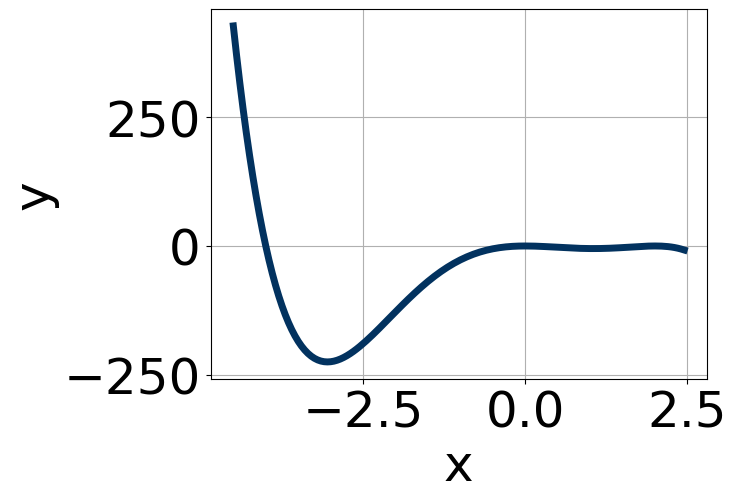
\includegraphics[width=0.5\textwidth]{../Figures/polyGraphToFunctionCopyC.png}
\end{center}
\begin{enumerate}[label=\Alph*.]
\item \( -20x^{4} (x - 2)^{8} (x + 4)^{11} \)
\item \( -4x^{8} (x - 2)^{11} (x + 4)^{7} \)
\item \( 6x^{4} (x - 2)^{6} (x + 4)^{8} \)
\item \( -7x^{8} (x - 2)^{5} (x + 4)^{8} \)
\item \( 14x^{6} (x - 2)^{10} (x + 4)^{7} \)

\end{enumerate} }
\litem{
Construct the lowest-degree polynomial given the zeros below. Then, choose the intervals that contain the coefficients of the polynomial in the form $x^3+bx^2+cx+d$.\[ -5 - 3 i \text{ and } -2 \]\begin{enumerate}[label=\Alph*.]
\item \( b \in [-1, 10], c \in [6.99, 8.99], \text{ and } d \in [7, 12] \)
\item \( b \in [-16, -10], c \in [53.47, 55.02], \text{ and } d \in [-72, -63] \)
\item \( b \in [-1, 10], c \in [4.6, 5.04], \text{ and } d \in [1, 7] \)
\item \( b \in [11, 13], c \in [53.47, 55.02], \text{ and } d \in [68, 69] \)
\item \( \text{None of the above.} \)

\end{enumerate} }
\litem{
Which of the following equations \textit{could} be of the graph presented below?
\begin{center}
    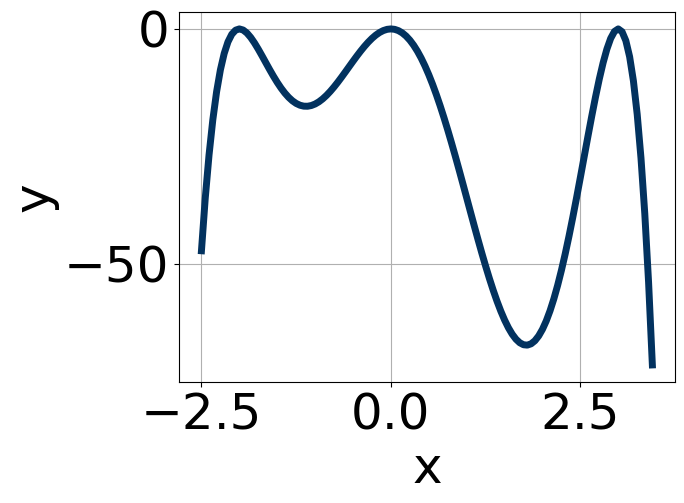
\includegraphics[width=0.5\textwidth]{../Figures/polyGraphToFunctionC.png}
\end{center}
\begin{enumerate}[label=\Alph*.]
\item \( -13x^{10} (x - 3)^{4} (x + 2)^{11} \)
\item \( 11x^{4} (x - 3)^{4} (x + 2)^{4} \)
\item \( -17x^{4} (x - 3)^{10} (x + 2)^{4} \)
\item \( -8x^{8} (x - 3)^{7} (x + 2)^{7} \)
\item \( 12x^{10} (x - 3)^{10} (x + 2)^{11} \)

\end{enumerate} }
\litem{
Describe the zero behavior of the zero $x = 3$ of the polynomial below.\[ f(x) = 5(x - 3)^{5}(x + 3)^{10}(x + 9)^{6}(x - 9)^{10} \]\begin{enumerate}[label=\Alph*.]
\begin{multicols}{2}\item 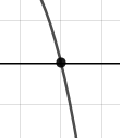
\includegraphics[width = 0.3\textwidth]{../Figures/polyZeroBehaviorAC.png}\item 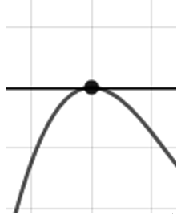
\includegraphics[width = 0.3\textwidth]{../Figures/polyZeroBehaviorBC.png}\item 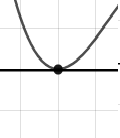
\includegraphics[width = 0.3\textwidth]{../Figures/polyZeroBehaviorCC.png}\item 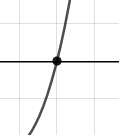
\includegraphics[width = 0.3\textwidth]{../Figures/polyZeroBehaviorDC.png}\end{multicols}\item None of the above.
\end{enumerate} }
\litem{
Describe the end behavior of the polynomial below.\[ f(x) = 2(x + 7)^{3}(x - 7)^{8}(x - 2)^{2}(x + 2)^{4} \]\begin{enumerate}[label=\Alph*.]
\begin{multicols}{2}\item 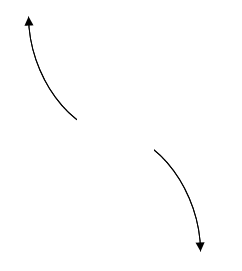
\includegraphics[width = 0.3\textwidth]{../Figures/polyEndBehaviorAC.png}\item 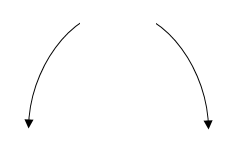
\includegraphics[width = 0.3\textwidth]{../Figures/polyEndBehaviorBC.png}\item 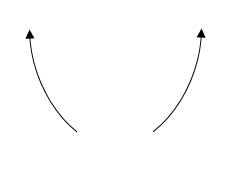
\includegraphics[width = 0.3\textwidth]{../Figures/polyEndBehaviorCC.png}\item 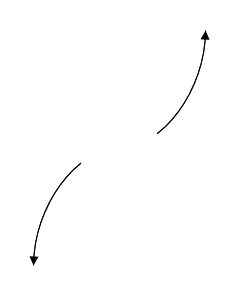
\includegraphics[width = 0.3\textwidth]{../Figures/polyEndBehaviorDC.png}\end{multicols}\item None of the above.
\end{enumerate} }
\litem{
Describe the end behavior of the polynomial below.\[ f(x) = -8(x - 9)^{4}(x + 9)^{5}(x + 2)^{4}(x - 2)^{5} \]\begin{enumerate}[label=\Alph*.]
\begin{multicols}{2}\item 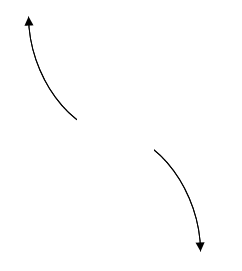
\includegraphics[width = 0.3\textwidth]{../Figures/polyEndBehaviorCopyAC.png}\item 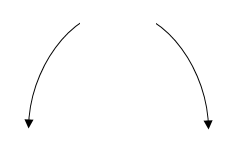
\includegraphics[width = 0.3\textwidth]{../Figures/polyEndBehaviorCopyBC.png}\item 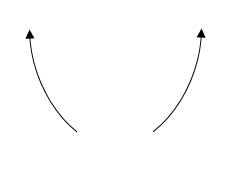
\includegraphics[width = 0.3\textwidth]{../Figures/polyEndBehaviorCopyCC.png}\item 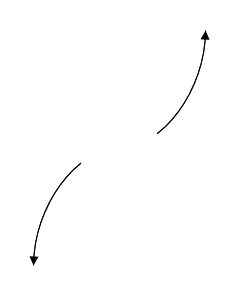
\includegraphics[width = 0.3\textwidth]{../Figures/polyEndBehaviorCopyDC.png}\end{multicols}\item None of the above.
\end{enumerate} }
\litem{
Construct the lowest-degree polynomial given the zeros below. Then, choose the intervals that contain the coefficients of the polynomial in the form $ax^3+bx^2+cx+d$.\[ \frac{-1}{4}, \frac{-1}{5}, \text{ and } \frac{4}{5} \]\begin{enumerate}[label=\Alph*.]
\item \( a \in [97, 105], b \in [-39, -33], c \in [-38, -27], \text{ and } d \in [2, 6] \)
\item \( a \in [97, 105], b \in [-125, -121], c \in [36, 47], \text{ and } d \in [-7, -2] \)
\item \( a \in [97, 105], b \in [-87, -79], c \in [-1, 8], \text{ and } d \in [2, 6] \)
\item \( a \in [97, 105], b \in [-39, -33], c \in [-38, -27], \text{ and } d \in [-7, -2] \)
\item \( a \in [97, 105], b \in [32, 40], c \in [-38, -27], \text{ and } d \in [2, 6] \)

\end{enumerate} }
\litem{
Construct the lowest-degree polynomial given the zeros below. Then, choose the intervals that contain the coefficients of the polynomial in the form $x^3+bx^2+cx+d$.\[ 3 - 3 i \text{ and } 4 \]\begin{enumerate}[label=\Alph*.]
\item \( b \in [-1, 7], c \in [-6, 0], \text{ and } d \in [-14, -11] \)
\item \( b \in [-1, 7], c \in [-8, -2], \text{ and } d \in [10, 13] \)
\item \( b \in [5, 20], c \in [34, 44], \text{ and } d \in [72, 78] \)
\item \( b \in [-10, -5], c \in [34, 44], \text{ and } d \in [-77, -69] \)
\item \( \text{None of the above.} \)

\end{enumerate} }
\end{enumerate}

\end{document}